\section{Results}

Based on the implementation described above the following is the overall algorithm which integrates all of the parts into a single command that represents what would be sent to the robots. 

%TC:ignore
\begin{tcolorbox}
\begin{itemize}
    \item[] For as long as the animal is not at the goal position:
\begin{enumerate}
    \item The animal makes a decision (and this decision is recorded)
    \item Non-non animal robot steps back from Non-animal robot
    \item Non-non animal robot path-finds to the path-finding target
    \item Non-animal robot steps back from Non-animal robot
    \item Non-animal robot path-finds to the path-finding target
    \item When both the robots are in the correct outer ring positions, they both move to the inner ring.
\end{enumerate}
\end{itemize}
\end{tcolorbox}
%TC:endignore
\subsection{Maze Loop}
\label{function:maze_loop}

After instantiating the environment (See Function \ref{function:instantiation}), the function which implements the logic described in Section \ref{section:implementation} must be executed in the following way. This corresponds to the diagrammatic representation of the algorithm described in Section \ref{fig:control_flow_diagram}. 


%TC:ignore
\begin{algorithm}[H]
\caption{The sequence of steps that are required for the whole procedure}
\begin{algorithmic}[1]
\STATE \textbf{Let the animal make the choice. Then let the maze change the States of the robots} 
\bindent{}
    \STATE \textit{Animal} makes choice
	\STATE Change the class of all the robots based on this choice
	\STATE Set the position of the animal on top of animal choice
\eindent{}
\\ \textbf{Find the path-finding targets before movement occurs}
\bindent{}
	\STATE Get the \textit{NNAR} class and \textit{NAR} class
	\STATE Set the \textit{path-finding} targets of \textit{NNAR}
	\STATE Set the \textit{path-finding} target of \textit{NAR}
\eindent{}
\\ \textbf{Execute path-finding for robots}
\bindent{}
	\STATE NNAR step back from NAR
	\STATE and path-finding to path-finding target
	\STATE NAR step back from AR
to	\STATE and path-finding got path-finding target
\eindent{}
\\ \textbf{Move robots into the inner ring}
\bindent{}
	\STATE NAR and NNAR step into inner ring
\eindent{}


\end{algorithmic}
\end{algorithm}
%TC:endignore

\afterpage{
\begin{landscape}
\subsection{Control flow diagram of the algorithm}
\label{fig:control_flow_diagram}
\begin{figure}[H]
    \centering
    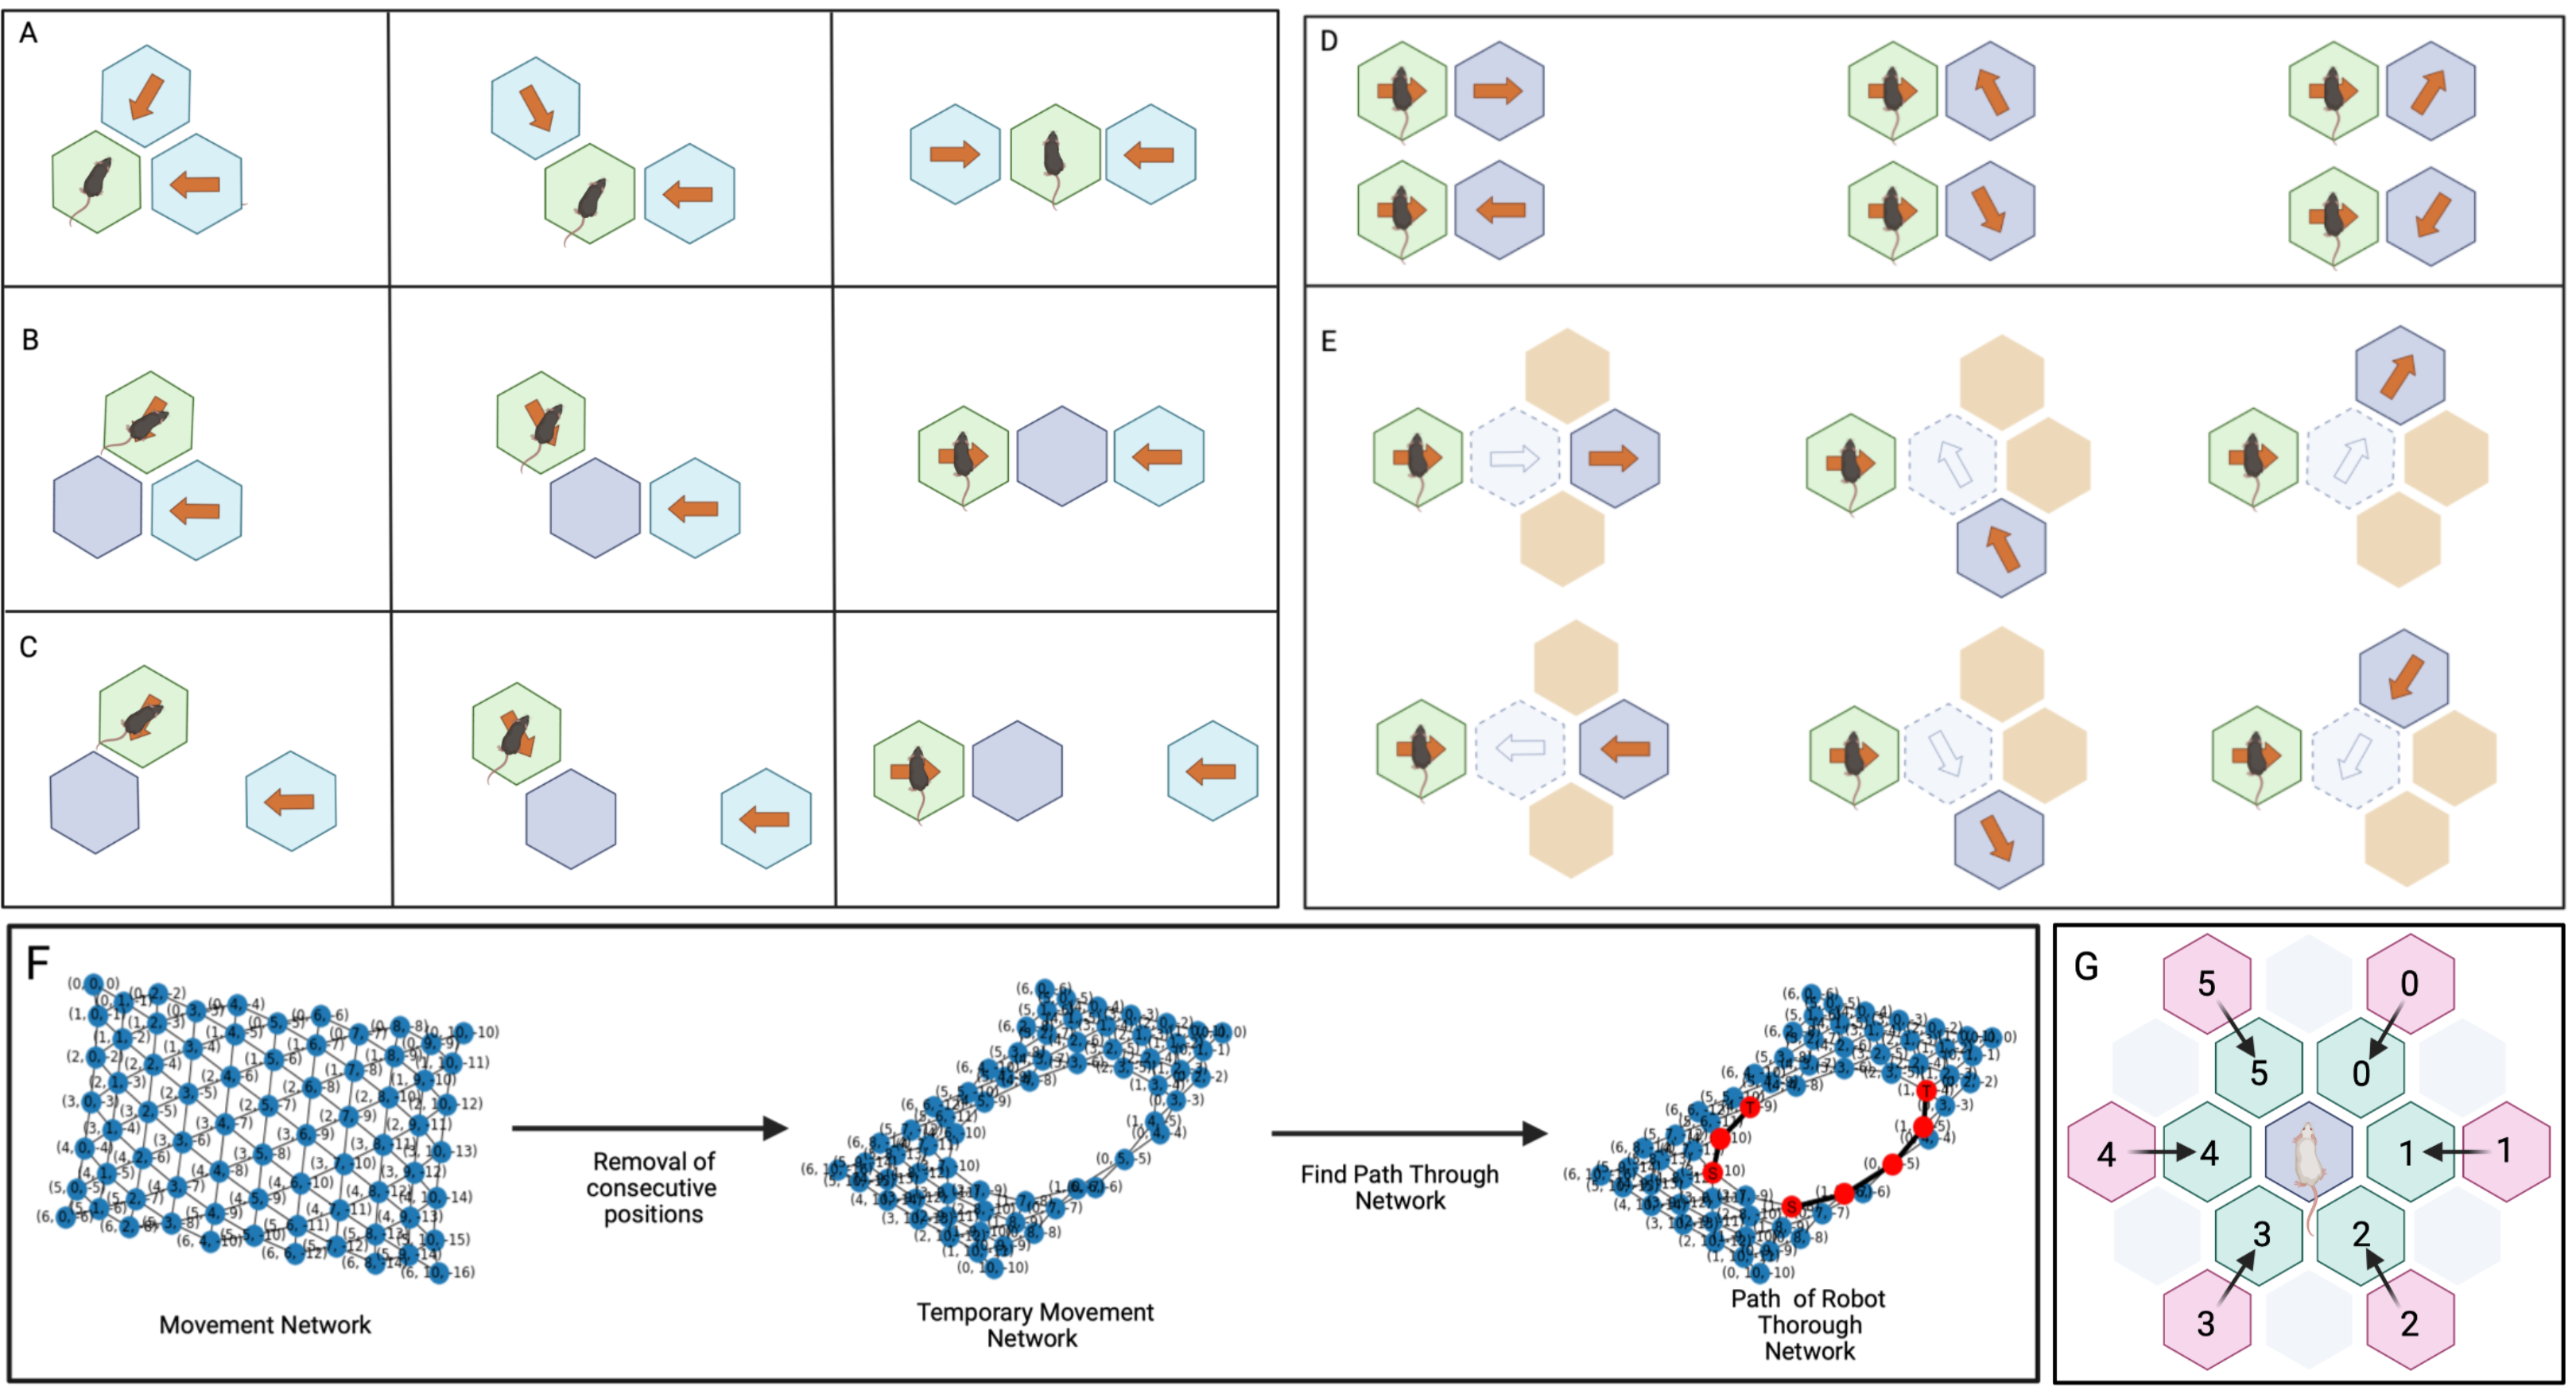
\includegraphics[scale = 0.786]{images/cfdl.png}
    \caption{Control Flow Diagram of algorithm implemented. \textbf{A} shows all possible states of the robot. The animal will decide which one to move to. Before this happens there is no difference between the \textit{NAR} and \textit{NNAR} so they are both coloured light blue. Once the animal has made a decision, the \textit{NAR} (in dark blue), the \textit{AR} (in green) and \textit{NNAR} robots (in light blue) are labeled appropriately. \textbf{C} shows that from all possible arrangements of the platforms, the \textit{NNAR} (light blue), must move backwards so that it does not intersect with the other robots when path-finding begins. \textbf{D} shows the two consecutive platforms, with all possible pairs of directions labeled. From \textbf{E}, it can be seen that for all the possible cases of the blue's orientation compared with the green, the \textit{NAR} must always move to the (orange) \textit{outer ring}. Once \textit{NNAR} and \textit{NAR} have reached the \textit{outer ring}, they must path-find to their path-finding target. \textbf{F} shows how this is achieved: The network of possible moves is generated, the moves that are inaccessible by the moving robot are removed from the network. Then the shortest path from the source to the target are found. \textbf{G} shows the final move required to get from the \textit{outer ring} of the target position to the (required) \textit{inner ring}.}

\end{figure}
\end{landscape}
}
